\begin{center}
\footnotesize\noindent\fbox{
	\parbox{\textwidth}{
	Utilizzare le functions degli esercizi precedenti per disegnare l'approssimazione della funzione \(\sin(x)\) nell'intervallo \([0, 2\pi]\), utilizzando le ascisse di interpolazione \(x_i=i\pi\), \(i= 0,1,2\).
	}
}\end{center}

\noindent Nell'immagine seguente si possono vedere i grafici della funzione \(f(x) = \sin(x)\) e dei tre polinomi interpolanti rispettivamente di Lagrange, Newton e di Hermite, tutti e tre calcolati fornendo in input alle funzioni precedentemente sviluppate le ascisse \(0, \pi, 2\pi \), la loro immagine attraverso \(f\) e, nel caso di Hermite, la loro immagine attraverso \(f'\).
\begin{center}
	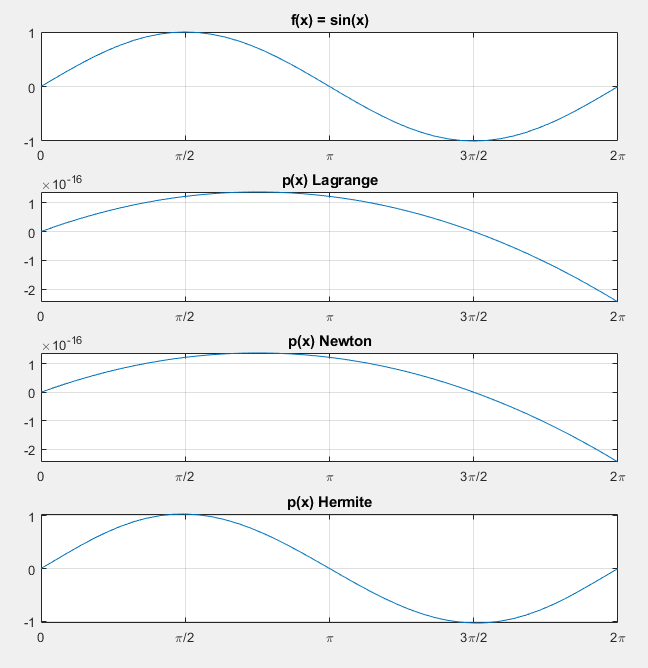
\includegraphics[scale=0.7]{cap4/4_4.png}
\end{center}
\noindent Come si nota facilmente, essendo \(f_i=0\) per tutte le nostre ascisse \(x_i\), il polinomio di Lagrange e di Newton in reallt\'a \'e semplicemente la retta \(y=0\). \\ \\
\noindent Il motivo per cui questo accade risulta particolarmente evidente considerando l'espressione del polinomio interpolante in forma di Lagrange: \( p(x) = \sum_{k=0}^{n}f_{k}L_{k,n}(x) \). Nel caso della forma di Newton, la situazione \'e ovviamente analoga, visto che le \(f_i\) nulle annullano le differenze divise, che vanno a loro volta ad annullare tutti i termini del polinomio. \\ \\
\noindent Di seguito il codice Matlab usato per realizzare i precedenti grafici.

\lstinputlisting[language=Matlab]{cap4/4_4.m}
